% !TeX program = xelatex
\documentclass{report}

\usepackage[margin=1cm,landscape]{geometry}
\usepackage{fontspec}
\defaultfontfeatures{Ligatures={NoCommon,%
NoDiscretionary,%
NoHistoric,%
NoRequired,%
NoContextual}}
\setsansfont{Carlito}[%
	SmallCapsFeatures={Letters=SmallCaps},%
	SmallCapsFont={Roboto},%
	ItalicFeatures={SmallCapsFont=Roboto-Italic},%
	BoldFeatures={SmallCapsFont=Roboto-Bold},%
	BoldItalicFeatures={SmallCapsFont=Roboto-BoldItalic}%
]

\usepackage{tikz}
\usepackage{tikz-cd}
\usetikzlibrary{%
	calc,%
	arrows.meta,%
	arrows,%
	automata,%
	overlay-beamer-styles,%
	snakes,%
	shapes.arrows,%
	shapes.geometric,%
	shapes.symbols,%
	fit,%
	positioning,%
	decorations.pathreplacing,%
	backgrounds,%
}
\tikzset{
	>=Triangle,
	nodes={align=center},
}

\definecolor{reddy}{RGB}{172, 0, 51}
\definecolor{dkred}{rgb}{.6, 0, 0}
\definecolor{dkgreen}{rgb}{0, .5, 0}
\definecolor{dkblue}{rgb}{0, 0, .5}
\definecolor{cred}{RGB}{219, 68, 55}
\definecolor{credlight}{RGB}{250, 227, 225}
\definecolor{cgreen}{RGB}{3, 148, 77}
\definecolor{cgreenlight}{RGB}{209, 251, 230}
\definecolor{cblue}{RGB}{2, 119, 189}
\definecolor{cbluelight}{RGB}{208, 237, 254}
\definecolor{corange}{RGB}{173, 128, 2}
\definecolor{corangelight}{RGB}{253, 219, 123}
\newcommand{\cblue}[1]{\textcolor{cblue}{#1}}
\newcommand{\bfcblue}[1]{\textcolor{cblue}{\textbf{#1}}}
\newcommand{\cred}[1]{\textcolor{cred}{#1}}
\newcommand{\bfcred}[1]{\textcolor{cred}{\textbf{#1}}}
\newcommand{\cgreen}[1]{\textcolor{cgreen}{#1}}
\newcommand{\bfcgreen}[1]{\textcolor{cgreen}{\textbf{#1}}}
\newcommand{\corange}[1]{\textcolor{corange}{#1}}
\newcommand{\bfcorange}[1]{\textcolor{corange}{\textbf{#1}}}

\usepackage{amsmath}
\usepackage{amsfonts}
\usepackage{amssymb}

\begin{document}
\sffamily

\section*{Infrastructure}

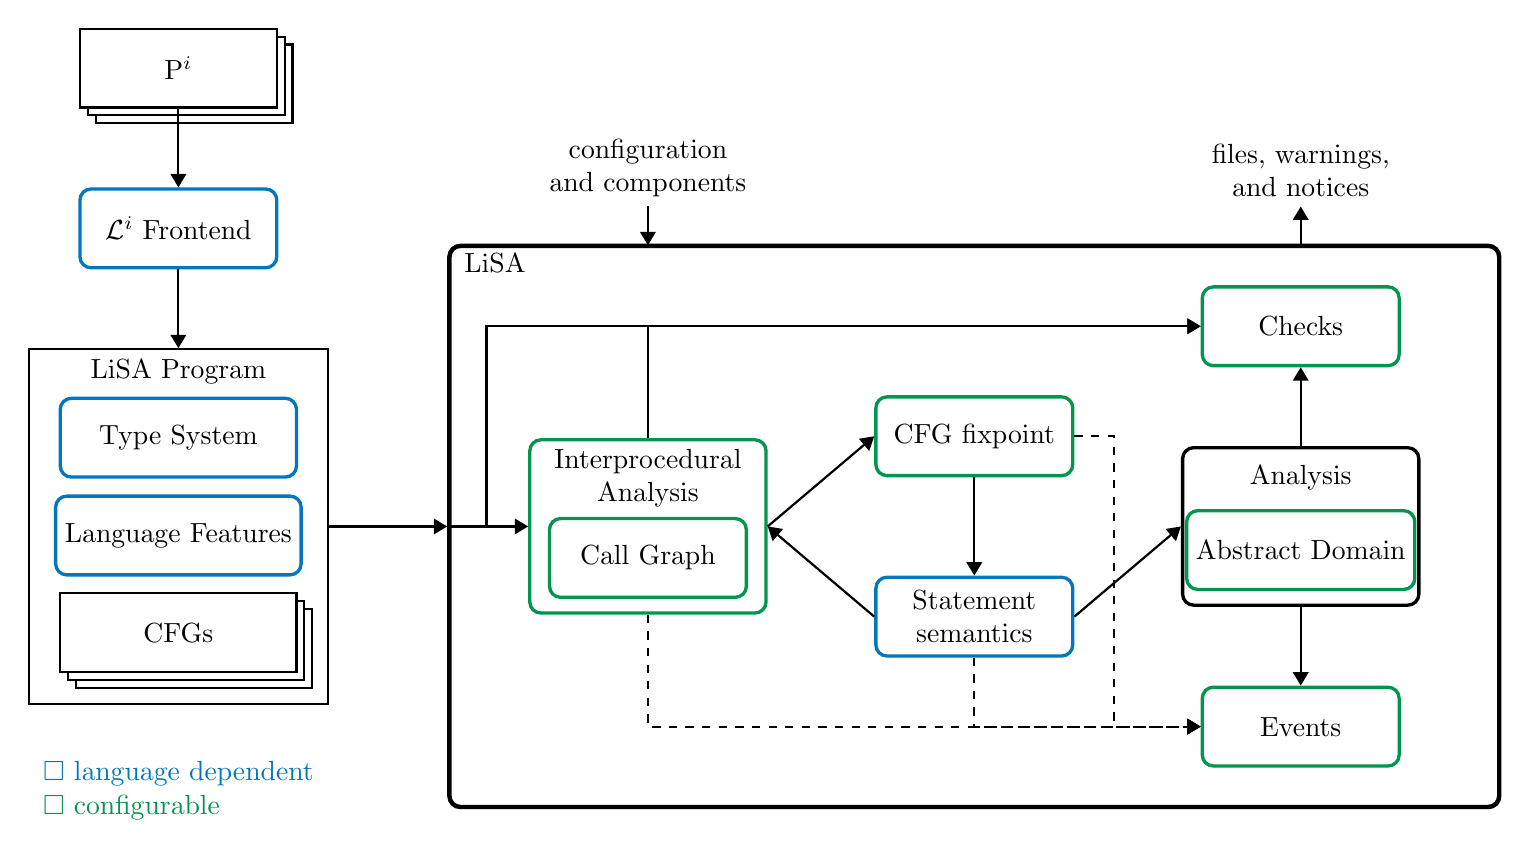
\begin{tikzpicture}[node distance=1cm,%
		comp/.style={draw, rectangle, very thick, rounded corners, minimum width=2.5cm, minimum height=1cm, fill=white},%
		input/.style={draw, rectangle, thick, minimum width=2.5cm, minimum height=1cm, fill=white}]
	\node (center) {};

	\node[comp, draw=cgreen] (fix) [above=.5cm of center] {CFG fixpoint};
	\node[comp, draw=cblue] (sem) [below=.5cm of center] {Statement\\semantics};

	\node[comp, minimum width=3cm, minimum height=2cm, text depth=1.3cm, draw=cgreen] (interproc) [left=2.5cm of center] {Interprocedural\\Analysis};
	\node[comp, anchor=south, draw=cgreen] (cg) at ($(interproc.south)+(0,0.2)$) {Call Graph};

	\node[comp, minimum width=3cm, minimum height=2cm, text depth=1.3cm] (state) [right=2.5cm of center] {Analysis};
	\node[comp, anchor=south, draw=cgreen] (domain) at ($(state.south)+(0,0.2)$) {Abstract Domain};

	\node[comp, draw=cgreen] (check) [above=of state] {Checks};
	\node[comp, draw=cgreen] (events) [below=of state] {Events};

	\draw[->, thick] (interproc.east) to (fix.west);
	\draw[->, thick] (fix) to (sem);
	\draw[->, thick] (sem.west) to (interproc.east);
	\draw[->, thick] (sem.east) to (state.west);
	\draw[->, thick] (state) to (check);
	\draw[->, thick] (state) to (events);
	\draw[->, thick] (interproc.north) |- (check.west);
	\draw[->, thick, dashed] (interproc.south) |- (events.west);
	\draw[->, thick, dashed] (sem.south) |- (events.west);
	\draw[->, thick, dashed] (fix.east) to ($(fix.east)+(0.5,0)$) |- (events.west);

	\node[comp, fill=none, ultra thick, fit=(fix)(state)(interproc)(check)(sem)(events), inner ysep=.5cm, inner xsep=1cm] (lisa) {};
	\node[anchor=north west, minimum width=1.2cm] at (lisa.north west) {LiSA};
	\draw[->, thick] (lisa.west) to ($(lisa.west)+(0.5,0)$) |- (interproc.west);
	\draw[->, thick] (lisa.west) to ($(lisa.west)+(0.5,0)$) |- (check.west);

	\node[anchor = south,] (out) [above=1cm of check]
	{files, warnings,\\and notices};
	\node[anchor = south] (conf) at (interproc |-,|- out.south) {configuration\\and components};
	\draw[->, thick] (conf.south) to ($(interproc.north)+(0,2.45)$);
	\draw[->, thick,] ($(check.north)+(0,0.5)$) to (out);

	\node[input, minimum width=3.8cm, minimum height=4.5cm, text depth=4cm] (pprog) [left=1.5cm of lisa] {LiSA Program};
	\node[input, minimum width=3cm, anchor=south] (cfgb1) at ($(pprog.south)+(0.2,0.2)$) {};
	\node[input, minimum width=3cm] (cfgb2) at ($(cfgb1)+(-0.1,0.1)$) {};
	\node[input, minimum width=3cm] (cfg) at ($(cfgb2)+(-0.1,0.1)$) {CFGs};
	\node[comp, anchor=south, draw=cblue, minimum width=3cm] (lf) at ($(cfg.north)+(0,0.2)$) {Language Features};
	\node[comp, anchor=south, draw=cblue, minimum width=3cm] (ts) at ($(lf.north)+(0,0.2)$) {Type System};

	\node[comp, draw=cblue] (frontend) [above=of pprog] {$\mathcal{L}^i$ Frontend};

	\node[input] (prog) [above=of frontend] {P$^i$};
	\begin{scope}[on background layer]
		\node[input] at ($(prog)+(0.2,-0.2)$) {};
		\node[input] at ($(prog)+(0.1,-0.1)$) {};
	\end{scope}

	\draw[->, thick] (pprog) to (lisa);
	\draw[->, thick] (prog) to (frontend);
	\draw[->, thick] (frontend) to (pprog);

	\node[align=left] [below=of cfg]
	{\cblue{$\Box$ language dependent}\\\cgreen{$\Box$ configurable}};
\end{tikzpicture}

\end{document}
